% ── Section: Main Content ─────────────────────────────────────────────────────
\section{Main Content}

% ── Text + block ──────────────────────────────────────────────────────────────
\begin{frame}{Key Concept}
  \begin{block}{Definition}
    A concise, clear definition of the central concept.
  \end{block}

  \vspace{0.5em}
  Supporting explanation with more detail. You can reference
  prior work~\parencite{example2024}.

  \begin{alertblock}{Important}
    Highlight critical information here.
  \end{alertblock}
\end{frame}

% ── Two-column layout ─────────────────────────────────────────────────────────
\begin{frame}{Approach}
  \begin{columns}[T]
    \begin{column}{0.48\textwidth}
      \textbf{Method A}
      \begin{itemize}
        \item Step 1
        \item Step 2
        \item Step 3
      \end{itemize}
    \end{column}
    \hfill
    \begin{column}{0.48\textwidth}
      \textbf{Method B}
      \begin{itemize}
        \item Step 1
        \item Step 2
        \item Step 3
      \end{itemize}
    \end{column}
  \end{columns}
\end{frame}

% ── Table ─────────────────────────────────────────────────────────────────────
\begin{frame}{Comparison}
  \begin{table}
    \centering
    \begin{tabular}{lrr}
      \toprule
      Method      & Metric A & Metric B \\
      \midrule
      Baseline    & 72.3\%   & 1.45\,s  \\
      Ours (v1)   & 85.1\%   & 0.92\,s  \\
      Ours (v2)   & \textbf{91.4\%} & \textbf{0.78\,s} \\
      \bottomrule
    \end{tabular}
    \caption{Performance comparison across methods.}
  \end{table}
\end{frame}

% ── Code listing ──────────────────────────────────────────────────────────────
\begin{frame}[fragile]{Code Example}
  \begin{lstlisting}[language=Python, caption={A simple example}]
def hello_world():
    """Greet the world."""
    message = "Hello, pptex!"
    print(message)
    return message
  \end{lstlisting}
\end{frame}

% ── TikZ diagram ──────────────────────────────────────────────────────────────
\begin{frame}{Architecture}
  \begin{center}
    \begin{tikzpicture}[
      node distance=2cm,
      box/.style={rectangle, draw, rounded corners, minimum width=2.5cm,
                  minimum height=0.8cm, fill=pptexBlue!15}
    ]
      \node[box] (input)   {Input};
      \node[box] (process) [right of=input]  {Process};
      \node[box] (output)  [right of=process] {Output};

      \draw[->, thick] (input)   -- (process);
      \draw[->, thick] (process) -- (output);
    \end{tikzpicture}
  \end{center}
\end{frame}

% ── Chart ─────────────────────────────────────────────────────────────────────
\begin{frame}{Results}
  \begin{center}
    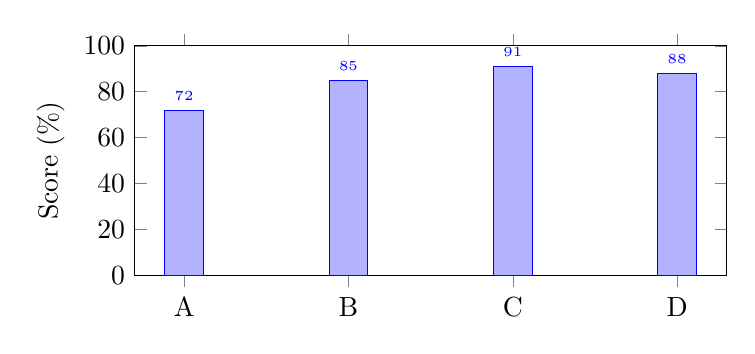
\begin{tikzpicture}
      \begin{axis}[
        width=0.75\textwidth, height=4.5cm,
        ybar, bar width=14pt,
        symbolic x coords={A, B, C, D},
        xtick=data,
        ylabel={Score (\%)},
        ymin=0, ymax=100,
        nodes near coords,
        nodes near coords align={vertical},
        every node near coord/.style={font=\tiny},
      ]
        \addplot coordinates {(A,72) (B,85) (C,91) (D,88)};
      \end{axis}
    \end{tikzpicture}
  \end{center}
\end{frame}
